% Supplementary figures

% \begin{figure}[H]
% \centering
% % Example figure placeholder
% \fbox{\parbox{0.7\textwidth}{
% \centering
% \vspace{2cm}
% [Figure placeholder]\\
% Include your figure here using:\\
% \texttt{\textbackslash includegraphics[width=\textbackslash textwidth]\{assets/figures/figure-name.pdf\}}
% \vspace{2cm}
% }}
% \caption{Example supplementary figure caption}
% \label{fig:supp-example}
% \end{figure}


\begin{figure}[H]
    \centering
    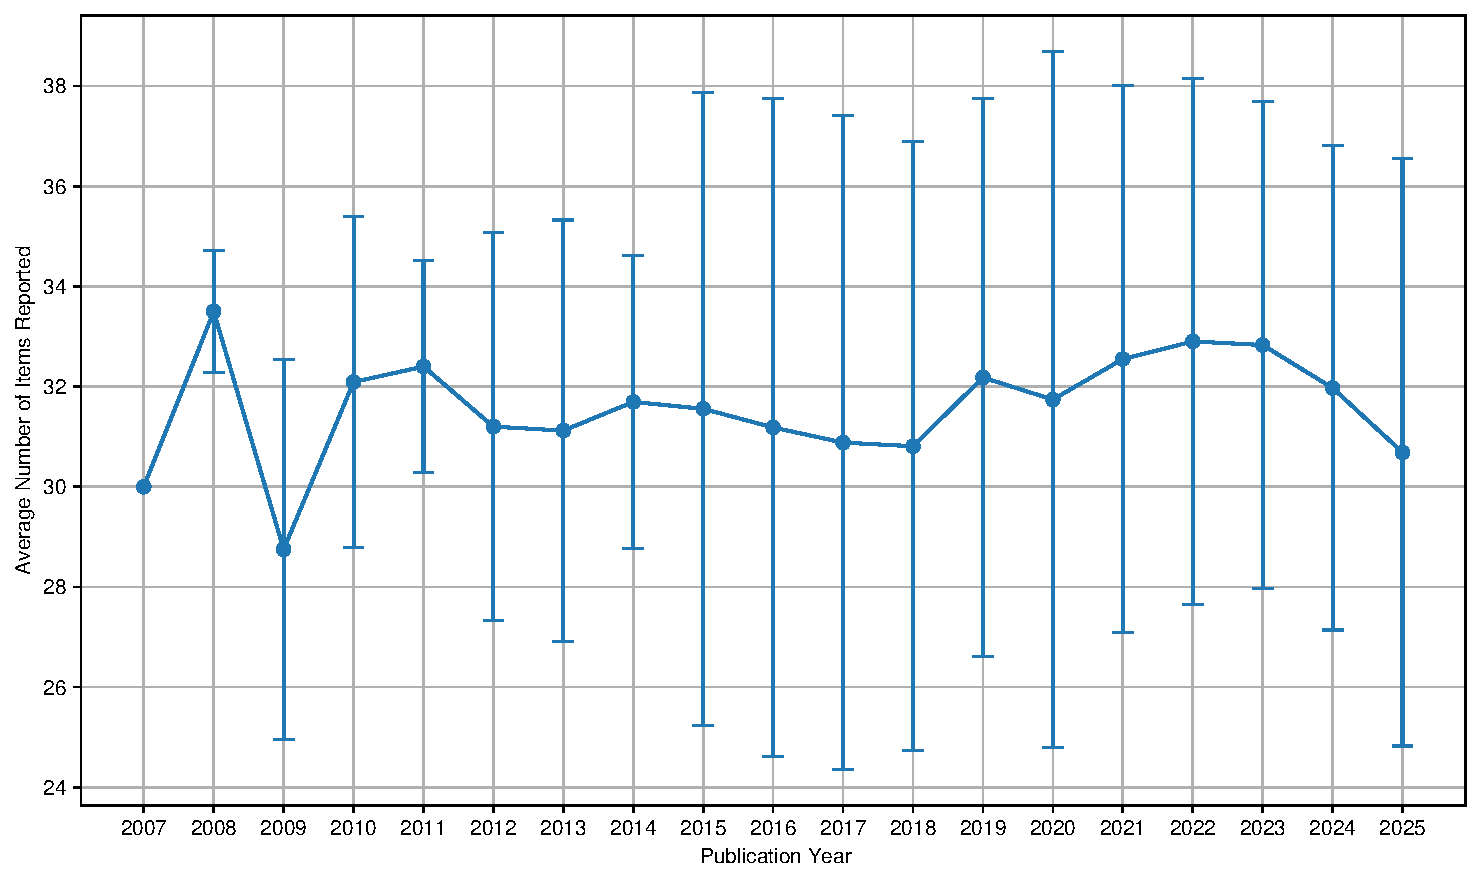
\includegraphics[width=0.8\linewidth]{assets/figures/subitem_any/avg_meet_num_by_year.pdf}
    \caption{Sensitivity analysis: STROBE-MR reporting by publication year}
    \label{append:fig:meet:year}
\end{figure}

\begin{figure}[H]
    \centering
    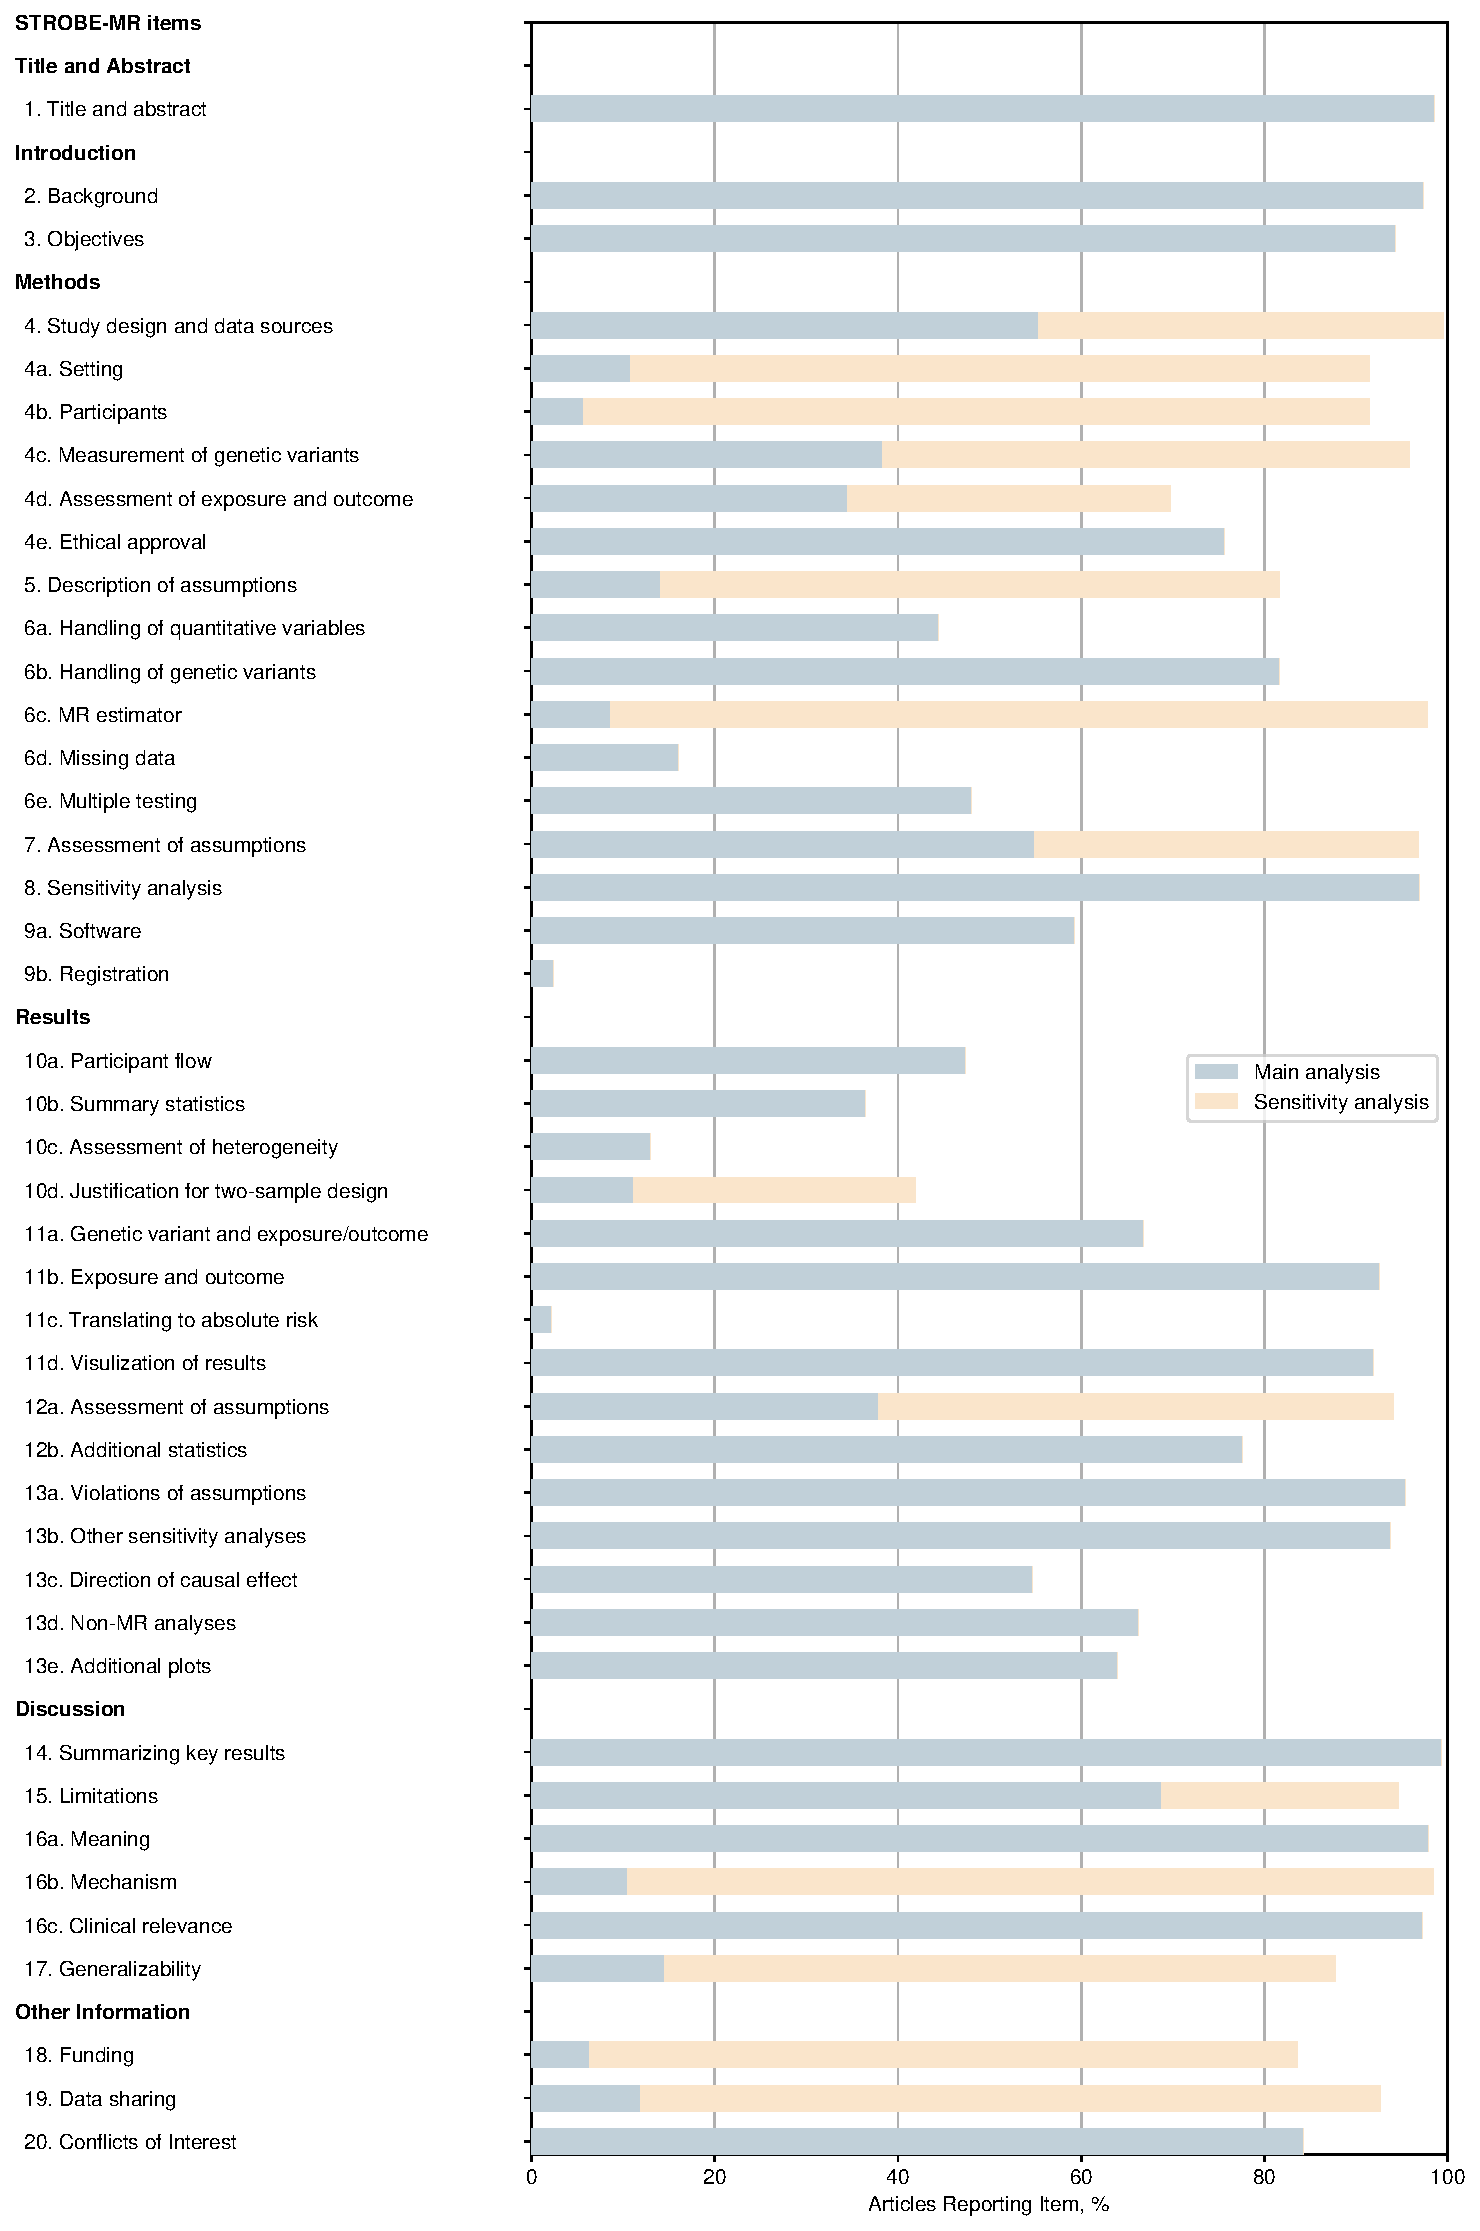
\includegraphics[width=0.8\linewidth]{assets/figures/subitem_any/meet_percentage_by_subitem.pdf}
    \caption{Sensitivity analysis: STROBE-MR reporting by item}
    \label{append:fig:meet:year}
\end{figure}

\begin{figure}[H]
    \centering
    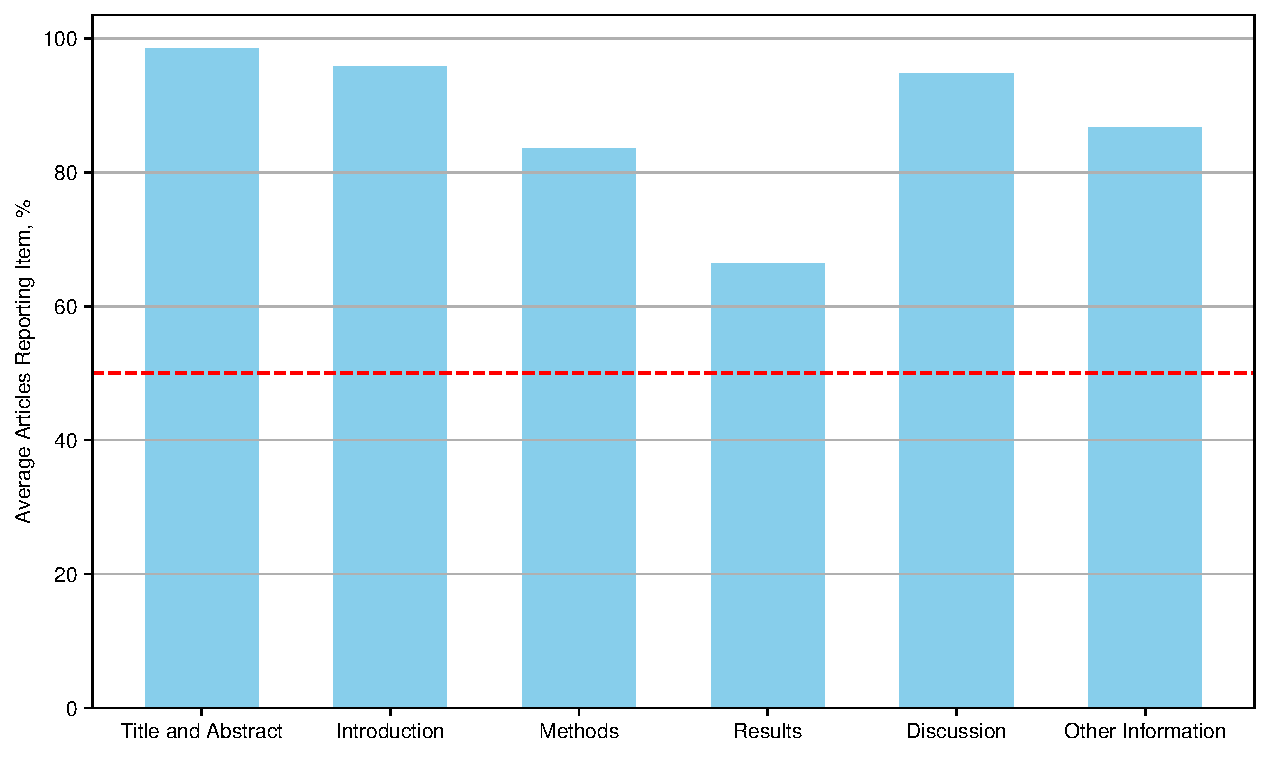
\includegraphics[width=0.8\linewidth]{assets/figures/subitem_any/meet_percentage_by_section.pdf}
    \caption{Sensitivity analysis: STROBE-MR reporting by section}
    \label{append:fig:meet:year}
\end{figure}


\begin{figure}[H]
    \centering
    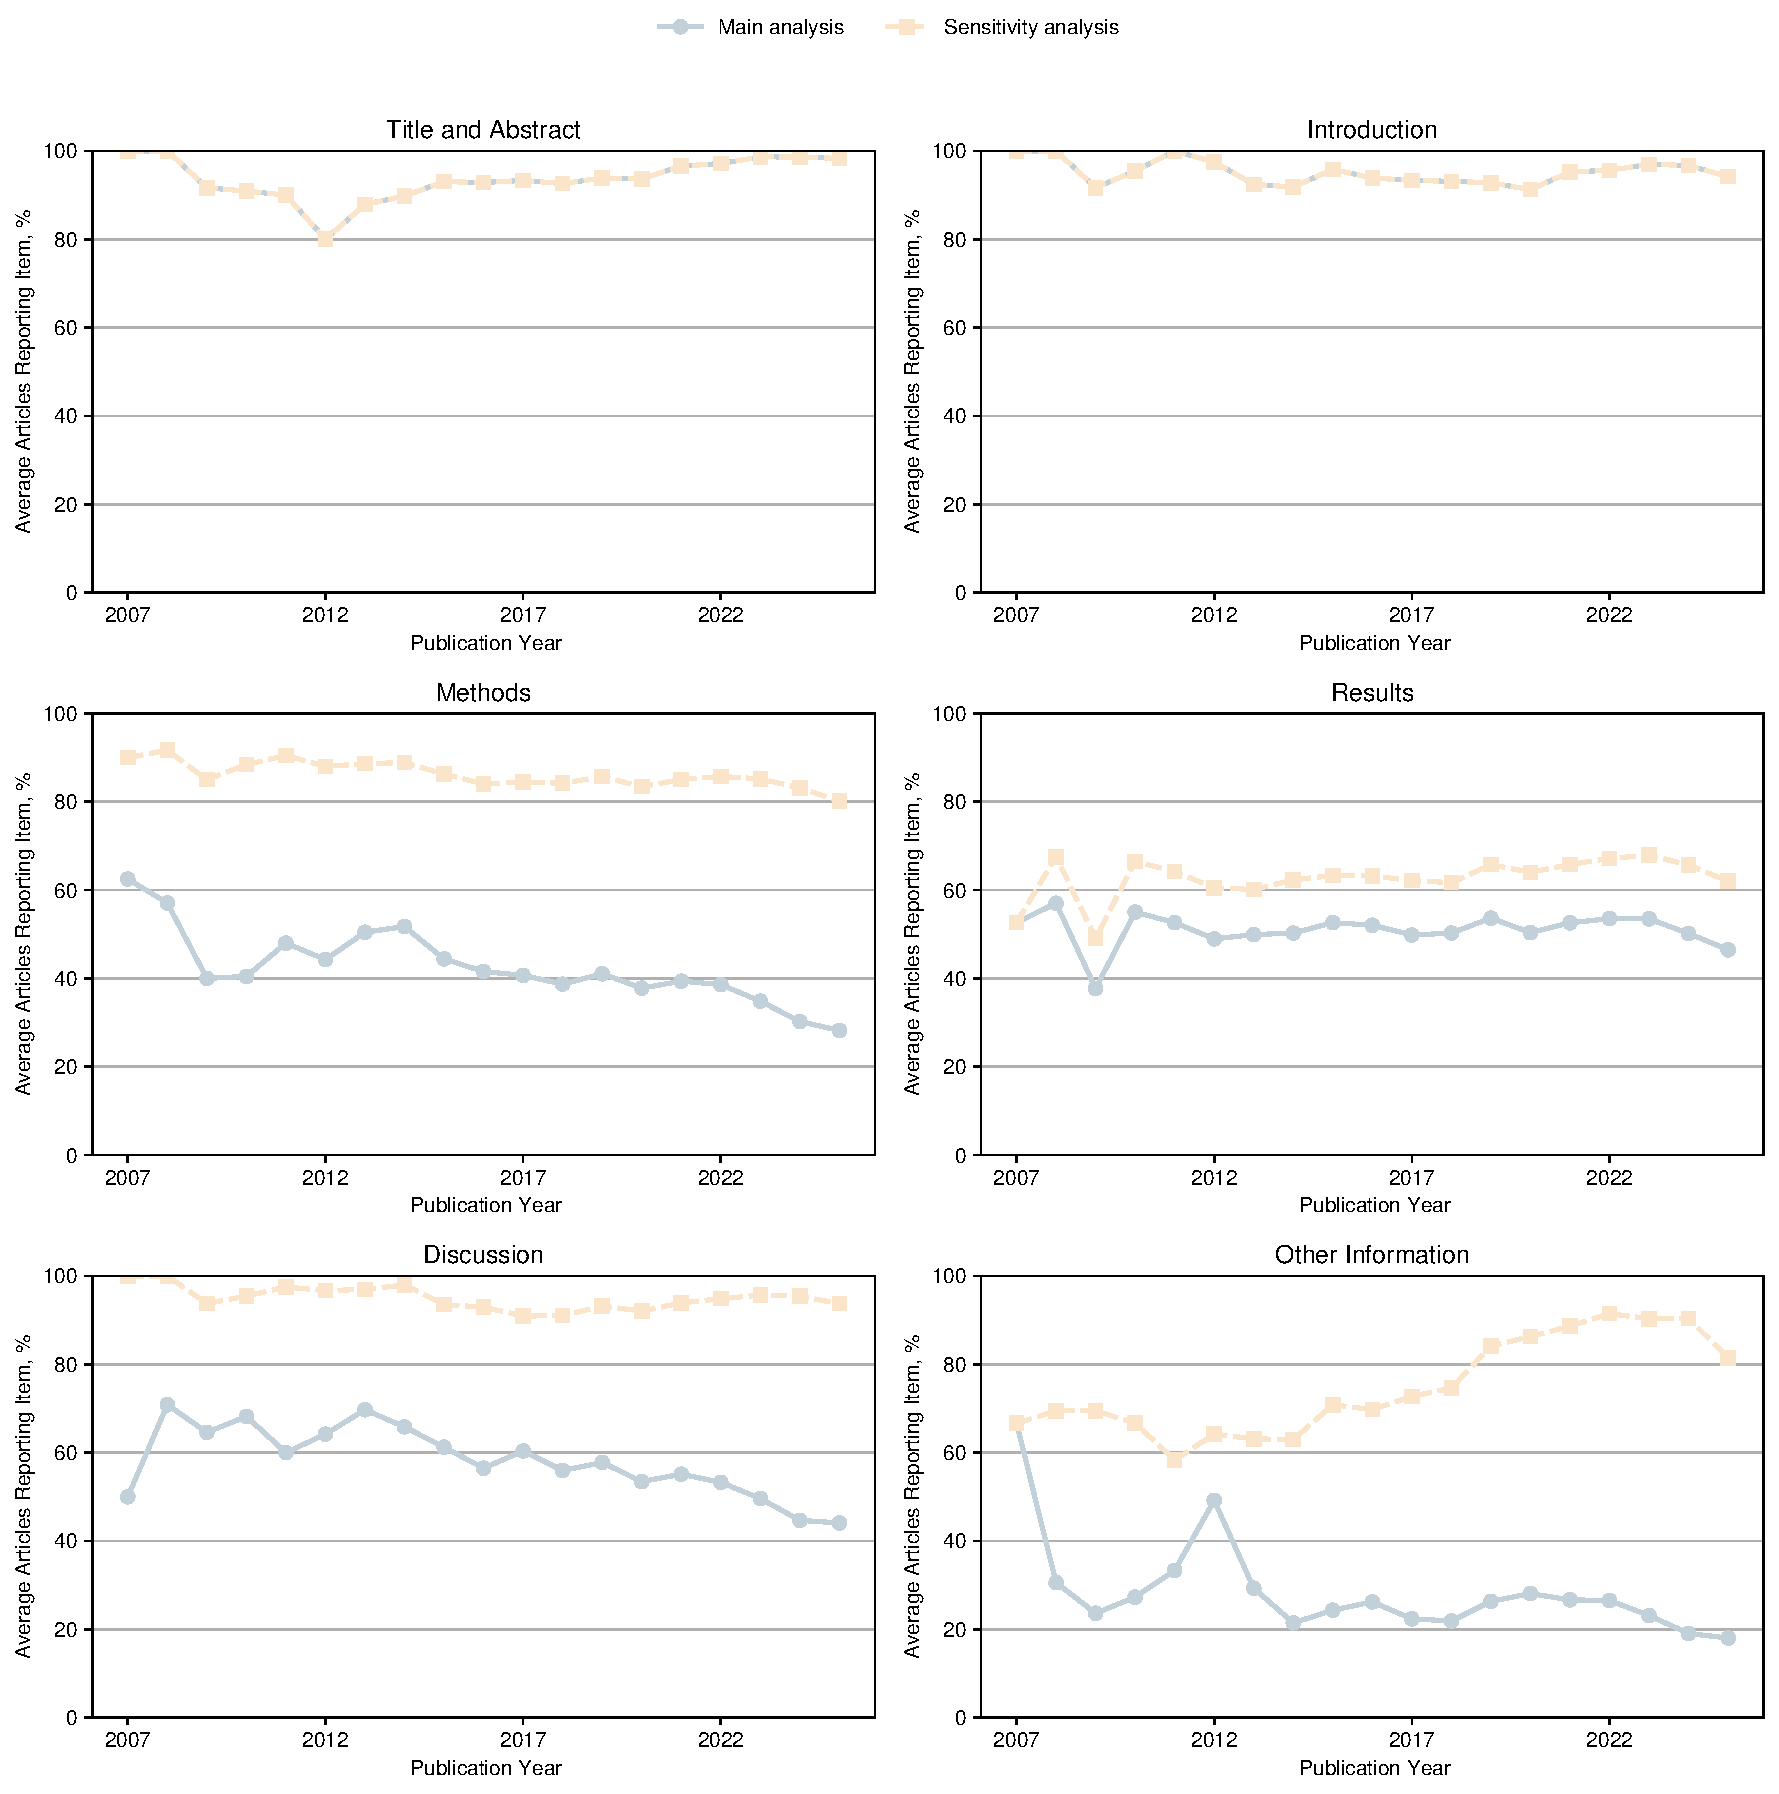
\includegraphics[width=0.8\linewidth]{assets/figures/subitem_any/meet_percentage_by_year_and_section.pdf}
    \caption{Sensitivity analysis: STROBE-MR reporting by year and section}
    \label{append:fig:meet:year}
\end{figure}

% Example cross-reference back to main manuscript
% This figure provides additional detail to Figure~\ref{fig:main-result} in the main manuscript.